%Model repurposing is common and it is done on a network scale \cite{traub} and an individual cell scale.
%Experimental evidence is starting to reveal that model re-purposing of pyramidal neurons might not be a good idea.
It is known that neural models and experimental measurements diverge generally and in important ways, however, it is desirable to know the specific sources of divergence. Models and experiments may disagree, for two reasons: A the model is not flexible enough to satisfy a particular constraint simultaneously to a collection of constraints, or, B the model was incorrectly fitted to the wrong type of measurement (for example model fitted to spike times at the expense of Rheobase, and FISlope). 

Since we don't yet have complete knowledge of model/experiment divergence, we don't necessarily know the best features to target with regards to model fitting. Specific knowledge of model/data disagreement facilitates the prioritized selection of features that should guide optimization. 
%a voltage recordings should be prioritized as optimization constraints.



\begin{figure}
    \centering
    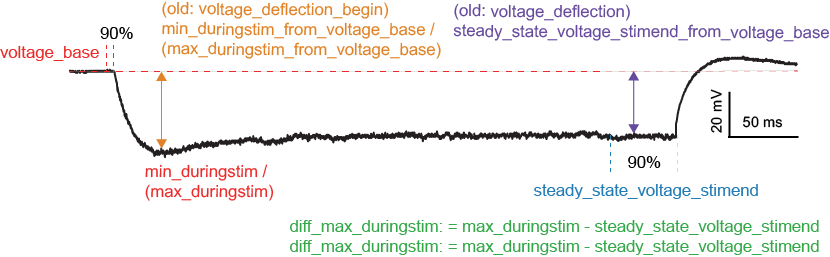
\includegraphics{figures/voltage_features.png}
    \caption{Caption}
    \label{fig:voltage_figures}
\end{figure}
\begin{figure}
    \centering
    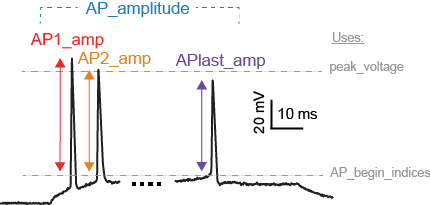
\includegraphics{figures/AP_Amplitude.png}
    \caption{Caption}
    \label{fig:features_example}
\end{figure}

\begin{figure}
    \centering
    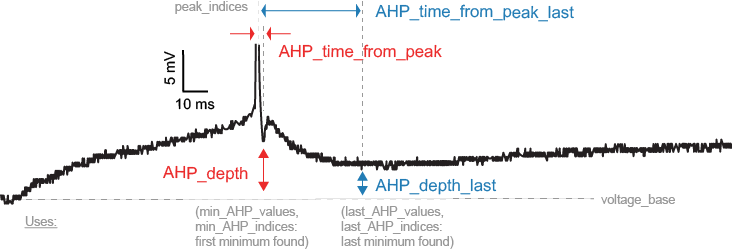
\includegraphics{figures/AHP.png}
    \caption{Caption}
    \label{fig:features_example_ahp}
\end{figure}



\subsubsection{Features} 
Consider a voltage recording at the location of the membrane of a neuron. Teams of researchers have already segmented voltage recordings into labelled sections, each section has a classification that is based on the shape of waveform in a limited region see figure \ref{fig:voltage_figures} for example. Rather than specifying by name each measurement it is often useful to refer collectively to these measurable shapes as "features". 

In the following multivariate analysis we analyze hundreds of such features, and we summarize important differences in a subset of this high dimensional feature space.  Below, I describe some neuronal model features that agreed well with experiments, and some features that diverged.


\subsubsection{Publications Associated with Model Sources}
972 models, 448 experiments.

Allen Institute for Brain Science Cell Types Database [7] can be accessed using the SDK. 

The Blue Brain Project Dataset can be obtained from the Data Navigator, or an API.

\begin{itemize}
\item Allen Institute V1 \cite{gouwens2018systematic}
\item Somatosensory Cortex \cite{markram2015} 
\end{itemize}

\subsubsection{Feature Extraction Libraries}
\begin{table}
\centering
%\resizebox{\textwidth}{!}{
\begin{tabular}{lll}
%\toprule
{} EFEL Ephys Feature Extraction Library & AllenSDK & Druckmann (2012) 
%\bottomrule
\end{tabular}
%}
\end{table}




\begin{tabular}{lll}
%\toprule
{} Injection 1 & Injection 2 & Injection 3 \\
 at $1.0 \times$ Rheobase & at $1.5 \times$ Rheobase & at $3.0 \times$ Rheobase 
%\bottomrule
\end{tabular}




%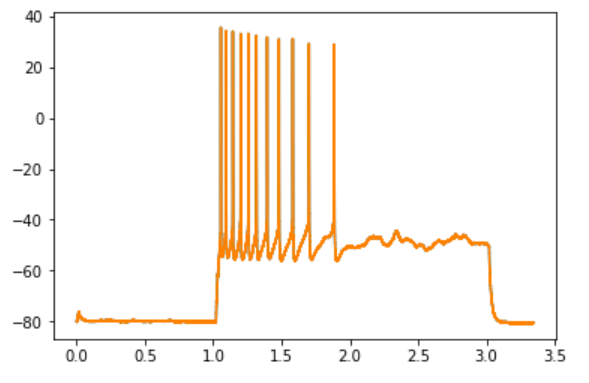
\includegraphics[]{chapters/app_tex/Allen_rush}
\begin{figure}
    \begin{center}
    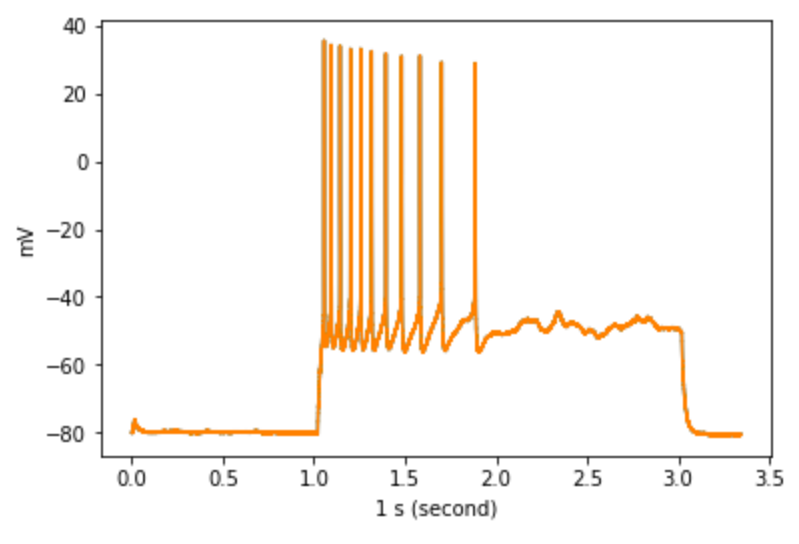
\includegraphics[width=0.6\linewidth]{figures/multi_spiking_large_allen}
    \caption{A voltage recording from a supra-threshold experiment waveform used as a basis for the Allen Brain Institute cell types data base. Publication Gouwens rat \cite{gouwens2018systematic}}
    \label{fig:adaptionm}
    \end{center}
\end{figure}    

\begin{figure}  
    \begin{center}
    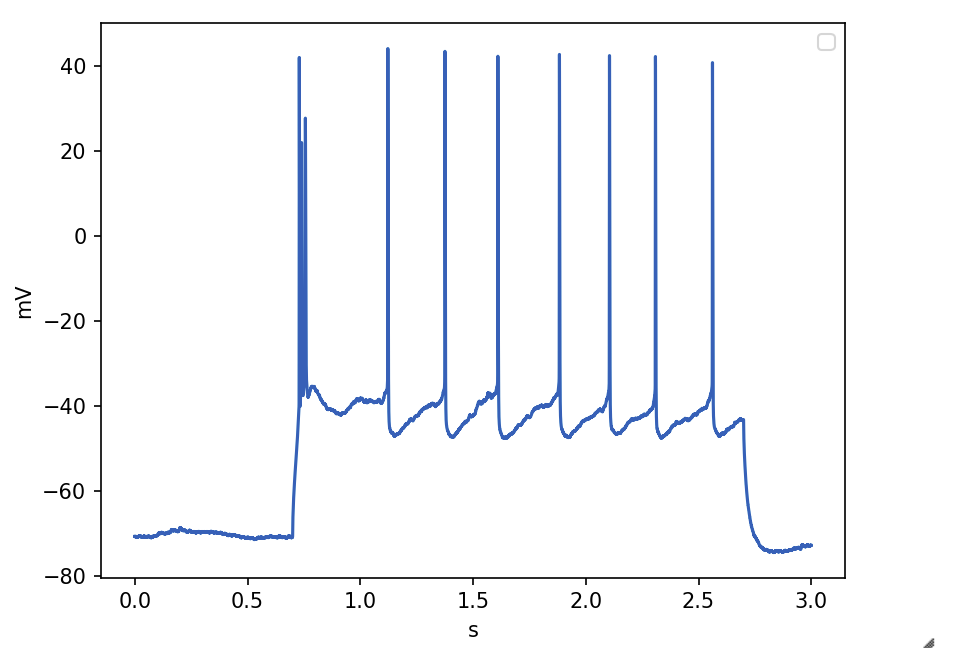
\includegraphics[width=0.6\linewidth]{figures/multi_spiking_large_bbp}
    \caption{Another example of a supra threshold experimental protocol. Publication Jouvanile rat \cite{toledo}}
    \label{fig:bbp_trace_adaption_late_spike}
    \end{center}
\end{figure}    

In order to identify electrical measurements or "features" that were responsible for the most variance in models and in-vitro, we performed Sparse Principle Component Analysis \cite{zou2006sparse} on the combined pool of model and in vitro experiments. 



\subsubsection{sources of disagreement}

The key advantage of using sparse PCA is the results are readily interpret able. A common sceanario in regular Principal Component Analysis is you may obtain a low dimensional embedding plot made from unit rotation vectors that maximize variance, but no way of relating the reduced dimensions back to the sources of variance in the system of interest. 

Sparse PCA yields an interpretable list of features, that build the principle components. This list of features is ranked and sorted with respect to their total contributions to the Eigen Vectors. Since two Eigen Vectors where made these are.

Principle component 1 had non zero loadings for ranked (highest to lowest)


The first Eigen Vector does not facilitate discrimination between models and experiments, but the second Eigen Vector spaces models and experiments into three seperate clusters.
$
upstroke_t_1.5x allen 
peak_t_1.5x allen 
threshold_t_1.5x allen 
fast_trough_t_1.5x allen 
fast_trough_t_3.0x allen 
upstroke_t_3.0x allen 
peak_t_3.0x allen 
threshold_t_3.0x allen 
peak_indices_1.5x efel 
min_AHP_indices_1.5x efel 
$


Principle component 2 had non zero loadings for ranked (highest to lowest)
$
fast_trough_index_1.5x allen 
peak_index_1.5x allen 
upstroke_index_1.5x allen 
threshold_index_1.5x allen 
fast_trough_index_3.0x allen 
peak_index_3.0x allen 
upstroke_index_3.0x allen 
threshold_index_3.0x allen
$
These are the weighted features that were used to make Eigen vectors 1 and 2, are responsible for most of the variance. Interestingly these features are mostly belonging to the Allen SDK, with two exceptions: $peak_indices_1.5x$ $min_AHP_indices_1.5 \times$ belonging to EFEL efel 

Move to Discussion 
Another observation is that a small majority of features used to create the sparse Eigen Vectors, are in the range of $1.5$ * rheobase, and slightly fewer are features from a $3.0\times$ rheobase experiment. I believe this is because, larger spike time variability $C_{V}$ is expressed in intermediate ranges of current injection. Under the highest current injections, high frequency evenly spaced spikes are likely, although spike frequency adaption is possible, the higher current may force to spikes to occur promptly after their refractory period, and in this case you might observe diminishing amplitude of spikes with increasing stimulus duration.

At $1.5 \times rheobase $ I believe there to be more spike time variation, at $3.0 \times rheobase $  I believe there to be more spike amplitude variation.


%Scientific insight is well-served by the discovery and optimization of abstract models that can reproduce experimental findings. NeuroML (NeuroML.org), a model description language for neuroscience, facilitates reproducibility and exchange of such models by providing an implementation-agnostic model description in a modular format. NeuronUnit (neuronunit.scidash.org) evaluates model accuracy by subjecting models to experimental data-driven validation tests, a formalization of the scientific method. 


% After applying dimensionality reduction to this very high dimensional feature space, we show that the real (biological neurons) and simulated (model neurons) recordings are easiley and fully discriminated by eye or any reasonable classifier.  

% Are they still discernable?
972 models, 448 experiments.

\subsubsection{Sparse PCA}
Interestingly models and experiments clustered separately to each other in the low dimensional space. That is to say models and data were easily separable in the direction of the 2nd Eigen Vector.

%The first principle component 
Models and experiments shared the same breadth of variability across the first principal component, with only slightly more variance in the experiments than in the data. Allen cell types experiments seemed to encompass the most variability out of models and experiments across all data sets.


Models clustered tightly and varied less

Sparse PCA revealed five overlapping different groups of neuronal identity's, and three non overlapping clusters.

Although imputation was successfully used to avoid dropping a large number of samples, about half of all initial BBP/Allen models data types were excluded from a final analysis, because they did not all capable of meeting inclusion criteria.  

There was one group of Allen cell type experiments that clustered on their own, making one set of the cluster.

sparse PCA 2nd Eigen Vector. 
%Consequently, not a single model neuron produced physiological responses that could be confused with a biological neuron. Was this a defect of the model design (e.g. key mechanisms unaccounted for) or of model parameterization? We found that if we introduced models that were revised via optimization the revised models overlapped with the distribution of biological neurons, and were mostly classified as such. The remaining post-optimization disagreement between models and biological neurons may reflect limitations of model design and can be investigated by probing the key features used by classifiers to distinguish these two populations. 

\begin{figure}    
\begin{center} 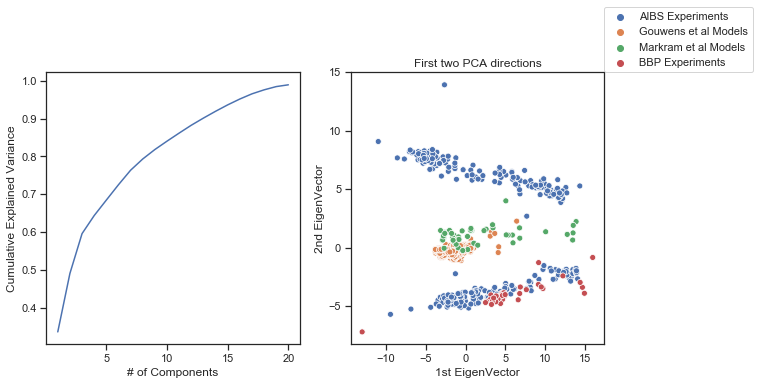
\includegraphics[width=1.0\linewidth]{figures/cortical_model_data_agreement_52_1}
    \caption{}
    \label{fig:}
\end{center}
\end{figure}    
\begin{figure}    
    \begin{center}
    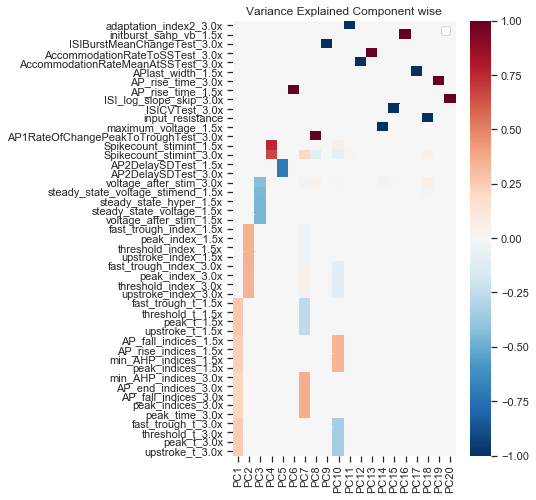
\includegraphics[width=1.0\linewidth]{figures/cortical_model_data_agreement_54_1.png}
    \caption{}
    \end{center}
\end{figure}    
\cite{wang2019sag}

\begin{figure}
    \centering
    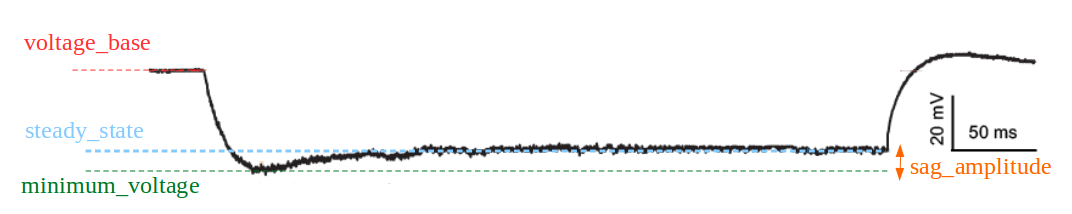
\includegraphics{figures/sag_amplitude}
    \caption{Caption}
    \label{fig:sag_amplitude}
\end{figure}

\begin{figure}
    \centering
    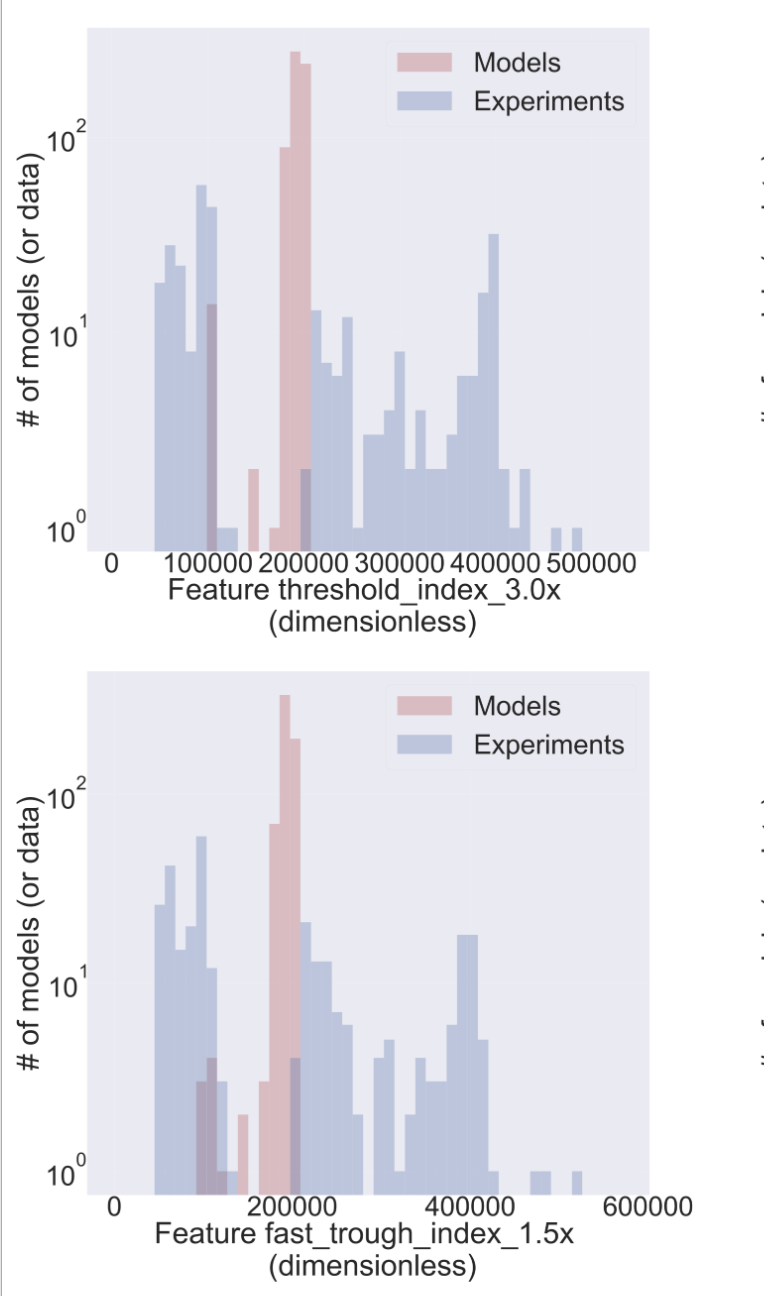
\includegraphics{figures/features_that_disagree}
    \caption{Caption}
    \label{fig:from_poster_disagree}
\end{figure}



\begin{itemize}
    \item upstroke\_t\_1.5x allen feature
    \item  peak\_t\_1.5x allen feature
    \item threshold\_t\_1.5x allen feature
    \item fast\_trough\_t\_1.5x allen feature
    \item fast\_trough\_t\_3.0x allen feature
    \item upstroke\_t\_3.0x allen feature
    \item peak\_t\_3.0x allen feature
    \item threshold\_t\_3.0x allen feature
    \item peak\_indices\_1.5x efel feature
    \item min\_AHP\_indices\_1.5x efel feature
\end{itemize}


\begin{itemize}

    \item fast\_trough\_index\_1.5x allen feature
    \item fast\_trough\_index\_3.0x allen feature
    \item threshold\_index\_1.5x allen feature
    \item peak\_index\_1.5x allen feature
    \item upstroke\_index\_1.5x allen feature
    \item peak\_index\_3.0x allen feature
    \item upstroke\_index\_3.0x allen feature
    \item threshold\_index\_3.0x allen feature
\end{itemize}


